% LuaLaTeX

\documentclass[a4paper, twoside, 12pt]{article}
\usepackage[latin]{babel} 
%\usepackage[landscape, left=3cm, right=1.5cm, top=2cm, bottom=1cm]{geometry} % okraje stranky
\usepackage[landscape, a4paper, mag=1166, truedimen, left=2cm, right=1.5cm, top=1.6cm, bottom=0.95cm]{geometry} % okraje stranky

\usepackage{fontspec}
\setmainfont[FeatureFile={junicode.fea}, Ligatures={Common, TeX}, RawFeature=+fixi]{Junicode}
%\setmainfont{Junicode}

% shortcut for Junicode without ligatures (for the Czech texts)
\newfontfamily\nlfont[FeatureFile={junicode.fea}, Ligatures={Common, TeX}, RawFeature=+fixi]{Junicode}

% Hebrew font:
% http://scripts.sil.org/cms/scripts/page.php?site_id=nrsi&id=SILHebrUnic2
\newfontfamily\hebfont[Scale=1]{Ezra SIL}

\usepackage{multicol}
\usepackage{color}
\usepackage{lettrine}
\usepackage{fancyhdr}

% usual packages loading:
\usepackage{luatextra}
\usepackage{graphicx} % support the \includegraphics command and options
\usepackage{gregoriotex} % for gregorio score inclusion
\usepackage{gregoriosyms}
\usepackage{wrapfig} % figures wrapped by the text
\usepackage{parcolumns}
\usepackage[contents={},opacity=1,scale=1,color=black]{background}
\usepackage{tikzpagenodes}
\usepackage{calc}
\usepackage{longtable}
\usetikzlibrary{calc}

\setlength{\headheight}{14.5pt}

% Commands used to produce a typical "Conventus" booklet

\newenvironment{titulusOfficii}{\begin{center}}{\end{center}}
\newcommand{\dies}[1]{#1

}
\newcommand{\nomenFesti}[1]{\textbf{\Large #1}

}
\newcommand{\celebratio}[1]{#1

}

\newcommand{\hora}[1]{%
\vspace{0.5cm}{\large \textbf{#1}}

\fancyhead[LE]{\thepage\ / #1}
\fancyhead[RO]{#1 / \thepage}
\addcontentsline{toc}{subsection}{#1}
}

% larger unit than a hora
\newcommand{\divisio}[1]{%
\begin{center}
{\Large \textsc{#1}}
\end{center}
\fancyhead[CO,CE]{#1}
\addcontentsline{toc}{section}{#1}
}

% a part of a hora, larger than pars
\newcommand{\subhora}[1]{
\begin{center}
{\large \textit{#1}}
\end{center}
%\fancyhead[CO,CE]{#1}
\addcontentsline{toc}{subsubsection}{#1}
}

% rubricated inline text
\newcommand{\rubricatum}[1]{\textit{#1}}

% standalone rubric
\newcommand{\rubrica}[1]{\vspace{3mm}\rubricatum{#1}}

\newcommand{\notitia}[1]{\textcolor{red}{#1}}

\newcommand{\scriptura}[1]{\hfill \small\textit{#1}}

\newcommand{\translatioCantus}[1]{\vspace{1mm}%
{\noindent\footnotesize \nlfont{#1}}}

% pruznejsi varianta nasledujiciho - umoznuje nastavit sirku sloupce
% s prekladem
\newcommand{\psalmusEtTranslatioB}[3]{
  \vspace{0.5cm}
  \begin{parcolumns}[colwidths={2=#3}, nofirstindent=true]{2}
    \colchunk{
      \input{#1}
    }

    \colchunk{
      \vspace{-0.5cm}
      {\footnotesize \nlfont
        \input{#2}
      }
    }
  \end{parcolumns}
}

\newcommand{\psalmusEtTranslatio}[2]{
  \psalmusEtTranslatioB{#1}{#2}{8.5cm}
}


\newcommand{\canticumMagnificatEtTranslatio}[1]{
  \psalmusEtTranslatioB{#1}{temporalia/extra-adventum-vespers/magnificat-boh.tex}{12cm}
}
\newcommand{\canticumBenedictusEtTranslatio}[1]{
  \psalmusEtTranslatioB{#1}{temporalia/extra-adventum-laudes/benedictus-boh.tex}{10.5cm}
}

% volne misto nad antifonami, kam si zpevaci dokresli neumy
\newcommand{\hicSuntNeumae}{\vspace{0.5cm}}

% prepinani mista mezi notovymi osnovami: pro neumovane a neneumovane zpevy
\newcommand{\cantusCumNeumis}{
  \setgrefactor{17}
  \global\advance\grespaceabovelines by 5mm%
}
\newcommand{\cantusSineNeumas}{
  \setgrefactor{17}
  \global\advance\grespaceabovelines by -5mm%
}

% znaky k umisteni nad inicialu zpevu
\newcommand{\superInitialam}[1]{\gresetfirstlineaboveinitial{\small {\textbf{#1}}}{\small {\textbf{#1}}}}

% pars officii, i.e. "oratio", ...
\newcommand{\pars}[1]{\textbf{#1}}

\newenvironment{psalmus}{
  \setlength{\parindent}{0pt}
  \setlength{\parskip}{5pt}
}{
  \setlength{\parindent}{10pt}
  \setlength{\parskip}{10pt}
}

%%%% Prejmenovat na latinske:
\newcommand{\nadpisZalmu}[1]{
  \hspace{2cm}\textbf{#1}\vspace{2mm}%
  \nopagebreak%

}

% mode, score, translation
\newcommand{\antiphona}[3]{%
\hicSuntNeumae
\superInitialam{#1}
\includescore{#2}

#3
}
 % Often used macros
%%%% Preklady jednotlivych zpevu (nektere se opakuji, a je dobre mit je
% vsechny na jedne hromade)

\newcommand{\trOratioAnteOfficium}{\translatioCantus{Otevři, Pane, má ústa, abych chválil tvé svaté jméno.
Očisti mé srdce od všech marnivých, zvrácených a~jiných myšlenek, osvěť rozum, rozněť cit,
abych mohl důstojně, soustředěně a~zbožně recitovat a~vysloužil si být
vyslyšen před tváří tvé velebnosti. Skrze Krista…}}

\newcommand{\trOratioPostOfficium}{\translatioCantus{\textit{Následující modlitbu
opatřil pro ty, kdo ji zbožně vyřknou po hodinkách, zesnulý papež Lev X.
odpustky za hříchy vzniklé při konání hodinek z~lidské křehkosti. Říká se
vkleče.}
Svatosvaté a~nerozdílné Trojici, ukřižovanému lidství našeho Pána Ježíše
Krista, přeblažené a~přeslavné plodné neporušenosti vždy Panny Marie
i~souhrnu všech svatých buď ode všeho stvoření věčná chvála, čest a~sláva, nám
pak buď dáno odpuštění všech hříchů, po nekonečné věky věků. Amen.}}

% HOURS ---

\newcommand{\trAntI}{\translatioCantus{Jasné narození slavné Panny Marie,
z pokolení (dosl. ze semene) Abrahámova, vzešlé z kmene Judova, z rodu Davidova.}}
\newcommand{\trAntII}{\translatioCantus{Dnes je Narození svaté Panny 
Marie, jejíž předrahý život osvěcuje všechny církve.}}

\newcommand{\trAntIII}{\translatioCantus{Maria, jež vzešla 
z královského rodu, září; myslí i duchem ji zbožně prosíme, aby 
nám pomáhala svými přímluvami.}}

\newcommand{\trAntIV}{\translatioCantus{Srdcem i duchem pějme Kristu 
k slávě o této svaté slavnosti vznešené Rodičky Boží Marie.}}

\newcommand{\trAntV}{\translatioCantus{Příjemně \notitia{?} 
oslavujme Narození blahoslavené Marie,
aby se ona za nás přimlouvala u Pána Ježíše Krista.}}

\newcommand{\trCapituli}{\translatioCantus{Před věky, na počátku mě stvořil, potrvám věčně. Ve svatém Stanu jsem před ním konala službu.}}

\newcommand{\trRespVesp}{\translatioCantus{Buď zdráva, Maria,
plná milosti: \grestar{} Pán s tebou. \Vbardot{} Požehnaná jsi mezi ženami,
a požehnaný plod života (ve smyslu lůna, břicha) tvého.}}

\newcommand{\trVersus}{\translatioCantus{\Vbardot{} Dnes je Narození svaté Panny Marie. \Rbardot{} Jejíž předrahý život osvěcuje všechny církve.}}

\newcommand{\trAntMagnificatI}{\translatioCantus{Konejme památku
veledůstojného narození slavné Panny Marie,
jíž se dostalo mateřské důstojnosti bez ztráty panenské cudnosti.}}

% Tento preklad je vice nez nejisty a ani alternativy, ktere jsem
% videl, me nepresvedcily...
\newcommand{\trAntBenedictus}{\translatioCantus{Slavnostně slavme 
dnešní narození Marie, vždy Panny a Rodičky Boží: v něm se objevuje
vysokost trůnu (totiž Marie, trůnu Božího Syna), aleluja.}}

\newcommand{\trAntMagnificatII}{\translatioCantus{Tvé narození,
Bohorodičko Panno, vyhlásilo radost celému světu:
z tebe totiž vzešlo Slunce spravedlnosti, Kristus, náš Bůh:
jenž zrušil kletbu a dal nám požehnání: přemohl smrt a dal nám život věčný.}}

\newcommand{\trOrationis}{\translatioCantus{Prosíme tě, Bože, 
uděl svým služebníkům dar nebeské milosti,
aby těm, jimž slehnutím blahoslavené Panny vyvstal počátek spásy, 
slavnost k poctě jejího narození přinesla
rozhojnění pokoje.
Skrze tvého Syna, našeho Pána Ježíše Krista, který s tebou žije a kraluje,
Bůh, v jednotě Ducha svatého po všechny věky věků.}}

\newcommand{\trFideliumAnimae}{\translatioCantus{\Vbardot{} Duše věrných ať pro
milosrdenství Boží odpočívají v~pokoji. \Rbardot{} Amen.}}

% Completorium

\newcommand{\trJubeDomne}{\translatioCantus{Rač, pane, požehnat.}}

\newcommand{\trComplBenedictio}{\translatioCantus{Pokojnou noc a~svatou smrt
nechť nám dopřeje všemohoucí Pán. \Rbardot{} Amen.}}

\newcommand{\trComplLectioBr}{\translatioCantus{Buďte střízliví, bděte.
Váš protivník Ďábel obchází jako lev řvoucí a~hledá, koho by pohltil.
Postavte se proti němu pevní ve víře.  Ale ty, Pane, smiluj se nad námi.
\Rbardot{} Bohu díky.}}

\newcommand{\trComplAntI}{\translatioCantus{Rač se smilovati nade mnou,
Hospodine, a vyslyš mou modlitbu.}}

\newcommand{\trComplCapituli}{\translatioCantus{Jsi přece, Hospodine,
uprostřed nás a~jmenujeme se po tobě.  Neopouštěj nás, Pane, náš Bože.}}

\newcommand{\trRespCompl}{\translatioCantus{Do tvých rukou, Pane, \grestar{}
poroučím svého ducha. \Vbardot{} Ty mne zachráníš, Pane, Bože věrný.}}

\newcommand{\trComplVersus}{\translatioCantus{\Vbardot{} Střez mne jako zřítelnici oka,
aleluja. \Rbardot{} Ve stínu svých křídel uschovej mne, aleluja.}}

\newcommand{\trAntSalvaNos}{\translatioCantus{Ochraňuj nás, Pane, když
bdíme, a~buď s~námi, když spíme, ať bdíme s~Kristem a~odpočíváme v~pokoji.}}

\newcommand{\trComplOrationis}{\translatioCantus{Zavítej, prosíme, Pane, sem
do našeho příbytku a~daleko od něj zažeň všechny úklady nepřítele. Ať tu
bydlí tví svatí andělé a~tvoje požehnání buď nad ním stále. Skrze…}}

\newcommand{\trSalveRegina}{\translatioCantus{Zdrávas Královno, matko
milosrdenství, živote, sladkosti a naděje naše, buď zdráva!
K tobě voláme, vyhnaní synové Evy,
k tobě vzdycháme, lkajíce a plačíce
v tomto slzavém údolí.
A proto, orodovnice naše,
obrať k nám své milosrdné oči
a Ježíše, požehnaný plod života svého,
nám po tomto putování ukaž,
ó milostivá, ó přívětivá,
ó přesladká, Panno Maria!}}

\newcommand{\trOraProNobis}{\translatioCantus{\Vbardot{} 
Oroduj za nás, svatá Boží Rodičko,
\Rbardot{} aby nám Kristus dal účast na svých zaslíbeních.}}

% Matutinum

\newcommand{\trMatInvitatorium}{\translatioCantus{}}

\newcommand{\trMatVeniteA}{\translatioCantus{Pojďte, chvalme s~radostí Pána,
s~jásotem slavme Boha, svou spásu; předstupme před tvář jeho s~díky, písně plesu pějme jemu.}}

\newcommand{\trMatVeniteB}{\translatioCantus{Neboť Bůh veliký jest Hospodin, a~král nade všecky bohy.
Jsouť v~jeho ruce všecky hlubiny země, temena hor jsou majetek jeho.}}

\newcommand{\trMatVeniteC}{\translatioCantus{Jehoť jest moře, neb on je učinil; i~souš
je dílo jeho rukou. Pojďme, klanějme se, padněme, klekněme před Pánem, svým
tvůrcem. Jeť on Pán, náš Bůh, a~my jsme lid, jejž on vodí a~ovce, jež pase.}}

\newcommand{\trMatVeniteD}{\translatioCantus{Kéž byste poslechli dnes hlasu jeho:
,,Nezatvrzujte svých srdcí jak v~Hádce, jak v~Pokušení na poušti, kde vaši otcové pokoušeli mne,
zkoušeli mne, ač vídali skutky mé.``}}

\newcommand{\trMatVeniteE}{\translatioCantus{Čtyřicet roků mrzel jsem se na to pokolení
a~řekl jsem: ,,Lid je to myslí stále bloudící``! Oni však nechtěli znáti mé cesty, takže jsem
přisáhl ve svém hněvu: ,,Nedojdou odpočinku mého!\mbox{}``}}

\newcommand{\trMatAntI}{\translatioCantus{}}

\newcommand{\trMatAntII}{\translatioCantus{}}

\newcommand{\trMatAntIII}{\translatioCantus{}}

\newcommand{\trMatVersusI}{\translatioCantus{}}

\newcommand{\trMatAbsolutioI}{\translatioCantus{Vyslyš Pane Ježíši Kriste
prosby svých služebníků \gredagger{} a~smiluj se nad námi, \grestar{} jenž
s~Otcem a~Duchem…}}

\newcommand{\trMatBenedictioI}{\translatioCantus{Rač, pane, požehnat.
Věčný Otec nám stále žehnej. \Rbardot{} Amen.}}

\newcommand{\trMatLecI}{\translatioCantus{Kéž by mě zulíbal polibky svých úst. 
Tvé milování je nad víno lahodnější;
vybraně voní tvé voňavky;
rozlévající se olej je tvé jméno,
proto tě dívky milují.
Strhni mě za sebou, poběžme!
Král mě uvedl do svých komnat;
budeš nám radostí a jásotem.
Víc než víno oslavíme tvé milování;
věru po právu jsi milován!
Snědá jsem, a přece krásná, jeruzalémské dcery,
jako stany kedarské,
jako šalmské závěsy.
}}

\newcommand{\trMatRespI}{\translatioCantus{}}

\newcommand{\trMatBenedictioII}{\translatioCantus{Rač, pane, požehnat.
Jednorozený Boží Syn nám žehnej \grestar{} a nám pomáhej. \Rbardot{} Amen.}}

\newcommand{\trMatLecII}{\translatioCantus{Nehleďte na mou osmahlou pleť:
to mě slunce ožehlo.
Synové mé matky se na mne rozzlobili,
poslali mě hlídat vinice.
A svou vinici, tu jsem nehlídala!
Pověz mi tedy, ty, jehož miluje mé srdce:
kam zavedeš své stádo pást,
kde ho necháš za poledne odpočívat?
Abych už nebloudila jako tulačka
poblíž stád druhů tvých.
Nevíš-li to, nejrásnější z žen,
jdi po stopách stáda
a kůzlata svá zaveď, ať se pasou
poblíž obydlí pastýřů.
Ke své klisně zapřažené do vozu faraonova
tebe, mé milá, přirovnávám.
Stále krásné jsou tvé líce s náušnicemi
i tvé hrdlo v náhrdelnících.}}

\newcommand{\trMatRespII}{\translatioCantus{}}

\newcommand{\trMatBenedictioIII}{\translatioCantus{Rač, pane, požehnat.
Milost Ducha Svatého ať osvítí nám smysly \grestar{} i srdce. \Rbardot{} Amen.}}

\newcommand{\trMatLecIII}{\translatioCantus{Zhotovíme ti zlaté náušnice
a kuličky ze stříbra.
Když král stoluje,
vydechuje můj nard svou vůni.
Můj milý je polštářek s myrhou,
jenž mi odpočívá mezi ňadry.
Můj milý je hrozen šáchoru
ve vinicích v Engadi.
Jak jsi krásná, milá moje,
jak jsi krásná!
Tvé oči jsou holubice.
Jak jsi krásný, můj milý,
jak líbezný!
Naše lože je samá zeleň.
Trámoví našeho domu je z cedru,
naše ostění z cypřiše.}}

\newcommand{\trMatRespIII}{\translatioCantus{}}

\newcommand{\trMatAntIV}{\translatioCantus{}}

\newcommand{\trMatAntV}{\translatioCantus{}}

\newcommand{\trMatAntVI}{\translatioCantus{}}

\newcommand{\trMatVersusII}{\translatioCantus{}}

\newcommand{\trMatAbsolutioII}{\translatioCantus{
Tvá milost a laskavost nechť nám pomáhá, jenž žiješ a vládneš s Otcem a Svatým Duchem na věky věků.}}

\newcommand{\trMatBenedictioIV}{\translatioCantus{Rač, pane, požehnat.
Bůh Otec všemohoucí, \grestar{} buď k nám milostivý a odpouštějící. \Rbardot{} Amen.}}

\newcommand{\trMatLecIV}{\translatioCantus{}}

\newcommand{\trMatRespIV}{\translatioCantus{}}

\newcommand{\trMatBenedictioV}{\translatioCantus{}}

\newcommand{\trMatLecV}{\translatioCantus{}}

\newcommand{\trMatRespV}{\translatioCantus{}}

\newcommand{\trMatBenedictioVI}{\translatioCantus{Rač, pane, požehnat.
Bůh rozněť v nás oheň své lásky. \Rbardot{} Amen.}}

\newcommand{\trMatLecVI}{\translatioCantus{}}

\newcommand{\trMatRespVI}{\translatioCantus{}}

\newcommand{\trMatAntVII}{\translatioCantus{}}

\newcommand{\trMatAntVIII}{\translatioCantus{}}

\newcommand{\trMatAntIX}{\translatioCantus{}}

\newcommand{\trMatVersusIII}{\translatioCantus{}}

\newcommand{\trMatAbsolutioIII}{\translatioCantus{Z okovů našich hříchů,
\grestar{} vysvoboď nás všemohoucí a milosrdný Pán. \Rbardot{} Amen.}}

\newcommand{\trMatBenedictioVII}{\translatioCantus{Rač, pane, požehnat.
Čtení evangelia nechť je nám \grestar{} spásou a ochranou. \Rbardot{} Amen.}}

\newcommand{\trMatLecVIIa}{\translatioCantus{
  Rodokmen Ježíše Krista, syna Davidova, syna Abrahámova:
  Abrahám zplodil Izáka,
  Izák zplodil Jakuba.}}

\newcommand{\trMatLecVIIb}{\translatioCantus{}}

\newcommand{\trMatRespVII}{\translatioCantus{}}

\newcommand{\trMatBenedictioVIII}{\translatioCantus{Rač, pane, požehnat.
\Rbardot{} Amen.}}

\newcommand{\trMatLecVIII}{\translatioCantus{}}

\newcommand{\trMatRespVIII}{\translatioCantus{}}

\newcommand{\trMatBenedictioIX}{\translatioCantus{Rač, pane, požehnat.
Do společnosti občanů nebes \grestar{} ať nás dovede král andělů.
\Rbardot{} Amen.}}

\newcommand{\trMatLecIX}{\translatioCantus{}}

% from the Czech Liturgia horarum
\newcommand{\trTeDeum}{\begin{translatioMulticol}{3}

Bože, tebe chválíme, 
tebe, Pane, velebíme.

Tebe, věčný Otče, 
oslavuje celá země.

Všichni andělé, 
cherubové i~serafové,

všechny mocné nebeské zástupy 
bez ustání volají:

Svatý, Svatý, Svatý, 
Pán, Bůh zástupů.

Plná jsou nebesa i~země 
tvé vznešené slávy.

Oslavuje tě 
sbor tvých apoštolů,

chválí tě 
velký počet proroků,

vydává o~tobě svědectví 
zástup mučedníků;

a~po celém světě 
vyznává tě tvá církev:

neskonale velebný, 
všemohoucí Otče,

úctyhodný Synu Boží, 
pravý a~jediný,

božský Utěšiteli, 
Duchu svatý.

Kriste, Králi slávy, 
tys od věků Syn Boha Otce;

abys člověka vykoupil, 
stal ses člověkem a~narodil ses z~Panny;

zlomil jsi osten smrti 
a~otevřel věřícím nebe;

sedíš po Otcově pravici 
a~máš účast na jeho slávě.

Věříme, že přijdeš soudit, 

a~proto tě prosíme:
přispěj na pomoc svým služebníkům, 
vždyť jsi je vykoupil svou předrahou krví;

dej, ať se radují s~tvými svatými 
ve věčné slávě.

Zachraň, Pane, svůj lid, žehnej svému dědictví, 
veď ho a~stále pozvedej.

Každý den tě budeme velebit 
a~chválit tvé jméno po všechny věky.

Pomáhej nám i~dnes, 
ať se nedostaneme do područí hříchu.

Smiluj se nad námi, Pane, 
smiluj se nad námi.

Ať spočine na nás tvé milosrdenství, 
jak doufáme v~tebe.

Pane, k~tobě se utíkáme, 
ať nejsme zahanbeni na věky. 
\end{translatioMulticol}}

\newcommand{\trMatEvangelium}{\translatioCantus{
  Rodokmen Ježíše Krista, syna Davidova, syna Abrahámova:
  Abrahám zplodil Izáka,
  Izák zplodil Jakuba,
  Jakub zplodil Judu a jeho bratry,
  Juda zplodil Farese a Zaru z Tamary,
  Fares zplodil Esroma,
  Esrom zplodil Arama,
  Aram zplodil Aminadaba,
  Aminadab zplodil Naasona,
  Naason zplodil Salmona,
  Salmon zplodil Boaze z Rahaby,
  Boaz zplodil Jobeda z Rut,
  Jobed zplodil Jessea,
  Jesse zplodil krále Davida.
  David zplodil Šalomouna z Uriášovy ženy,
  Šalomoun zplodil Roboama,
  Roboam zplodil Abiu,
  Abia zplodil Asu,
  Asa zplodil Josafata,
  Josafat zplodil Jorama,
  Joram zplodil Oziáše,
  Oziáš zplodil Joatama,
  Joatam zplodil Achaze,
  Achaz zplodil Ezechiáše,
  Ezechiáš zplodil Manasesa,
  Manases zplodil Amona,
  Amon zplodil Josiáše,
  Josiáš zplodil Jechoniáše a jeho bratry;
  tehdy došlo k odvlečení do Babylonu.
  Po odvlečení do Babylonu:
  Jechoniáš zplodil Salatiela,
  Salatiel zplodil Zorobabela,
  Zorobabel zplodil Abiuda,
  Abiud zplodil Eljakima,
  Eljakim zplodil Azora,
  Ator zplodil Sadoka,
  Sadok zplodil Achima,
  Achim zplodil Eliuda,
  Eliud zplodil Eleazara,
  Eleatar zplodil Matana,
  Matan zplodil Jakuba,
  Jakub zplodil Josefa, manžela Marie,
  z níž se narodil Ježíš, který se nazývá Kristus.}}

\newcommand{\trTeDecetLaus}{\translatioCantus{Tobě chvála, Tobě zpěvy, Tobě
sláva, Bohu Otci i~Synu i~Svatému Duchu, na věky věků. \Rbardot{} Amen.}}

% MASS ---

\newcommand{\trIntroitus}{\translatioCantus{Radujme se všichni
v Pánu, slavíce svátek ke cti Panny Marie: z něj se radují andělé
a spoluchválí Božího Syna. \textit{\color{red}Žl.} Má ústa vydala dobré slovo,
přednáším svá díla králi.}}

\newcommand{\trGraduale}{\translatioCantus{Požehnaná a ctihodná jsi,
Panno Maria: nedotčená (co do panenství) jsi byla shledána matkou
Spasitele. \Vbardot{} Panno Boží Rodičko, ten, jehož nepojme ani celý svět,
se uzavřel do tvých útrob, když se stal člověkem.}}

\newcommand{\trAlleluia}{\translatioCantus{Aleluja. \Vbardot{} Skvělá slavnost
slavné Panny Marie, z pokolení (dosl. ze semene) Abrahámova, vzešlé z kmene 
Judova, z rodu Davidova.}}

\newcommand{\trOffertorium}{\translatioCantus{Blažená jsi, Panno Maria,
tys nosila Stvořitele všeho; porodila jsi toho, který tě utvořil,
a na věky zůstáváš Pannou.}}

\newcommand{\trCommunio}{\translatioCantus{Budou mě blahoslavit
všechna pokolení, protože mi učinil veliké věci ten, který je mocný.}}

% LITTLE HOURS ---

\newcommand{\trVersusTertia}{\translatioCantus{\Vbardot{} \Rbardot{}}}

\newcommand{\trCapituliEtSic}{\translatioCantus{
Tak jsem se usadila na Sionu a v milovaném městě jsem nalezla odpočinek,
v Jeruzalémě vykonávám svou moc.
Zakořenila jsem u lidu plného slývy, na panství Páně, v jeho dědictví.}}

\newcommand{\trVersusSexta}{\translatioCantus{\Vbardot{} \Rbardot{}}}

\newcommand{\trCapituliInPlateis}{\translatioCantus{
Na planině jako skořicovník a akant jsem vydávala vůni, jako vybraná myrha
jsem voněla.}}

\newcommand{\trVersusNona}{\translatioCantus{\Vbardot{} \Rbardot{}}}
 % Czech translations of the proper texts

\newcommand{\annusEditionis}{2015}

\def\hebinitial#1{%
\leavevmode{\newbox\hebbox\setbox\hebbox\hbox{\hebfont{#1}\hskip 1mm}\kern -\wd\hebbox\hbox{\hebfont{#1}\hskip 1mm}}%
}

%%%% Vicekrat opakovane kousky

\newcommand{\anteOrationem}{
  \rubrica{Ante Orationem, cantatur a Superiore:}

  \pars{Supplicatio Litaniæ.}

  \gregorioscore{temporalia/supplicatiolitaniae.gtex}

  \pars{Oratio Dominica.}

  \gregorioscore{temporalia/oratiodominica.gtex}

  \rubrica{Deinde dicitur ab Hebdomadario:}

  \gregorioscore{temporalia/dominusvobiscum-solemnis.gtex}

  \rubrica{In choro monialium loco Dominus vobiscum dicitur:}

  \gregorioscore{temporalia/domineexaudi.gtex}
}

\newcommand{\tuAutem}{
  \vfill

  \gregorioscore{temporalia/tuautem.gtex}
}

\setlength{\columnsep}{30pt} % prostor mezi sloupci

%%%%%%%%%%%%%%%%%%%%%%%%%%%%%%%%%%%%%%%%%%%%%%%%%%%%%%%%%%%%%%%%%%%%%%%%%%%%%%%%%%%%%%%%%%%%%%%%%%%%%%%%%%%%%
\begin{document}

% Here we set the space around the initial.
% Please report to http://home.gna.org/gregorio/gregoriotex/details for more details and options
\grechangedim{afterinitialshift}{2.2mm}{scalable}
\grechangedim{beforeinitialshift}{2.2mm}{scalable}

\grechangedim{interwordspacetext}{0.32 cm plus 0.15 cm minus 0.05 cm}{scalable}%
\grechangedim{annotationraise}{-0.2cm}{scalable}

% Here we set the initial font. Change 38 if you want a bigger initial.
% Emit the initials in red.
\grechangestyle{initial}{\color{red}\fontsize{38}{38}\selectfont}

\pagestyle{empty}

%%%% Titulni stranka
\begin{titulusOfficii}
\dies{Die 8. Septembris.}
\nomenFesti{In Nativitate B. Mariæ Virginis.}
\celebratio{Duplex 2. classis.} % puvodne "cum Octava." Oktavy byly ale zruseny
\end{titulusOfficii}

% graphic
\vspace{1.5cm}
\begin{center}
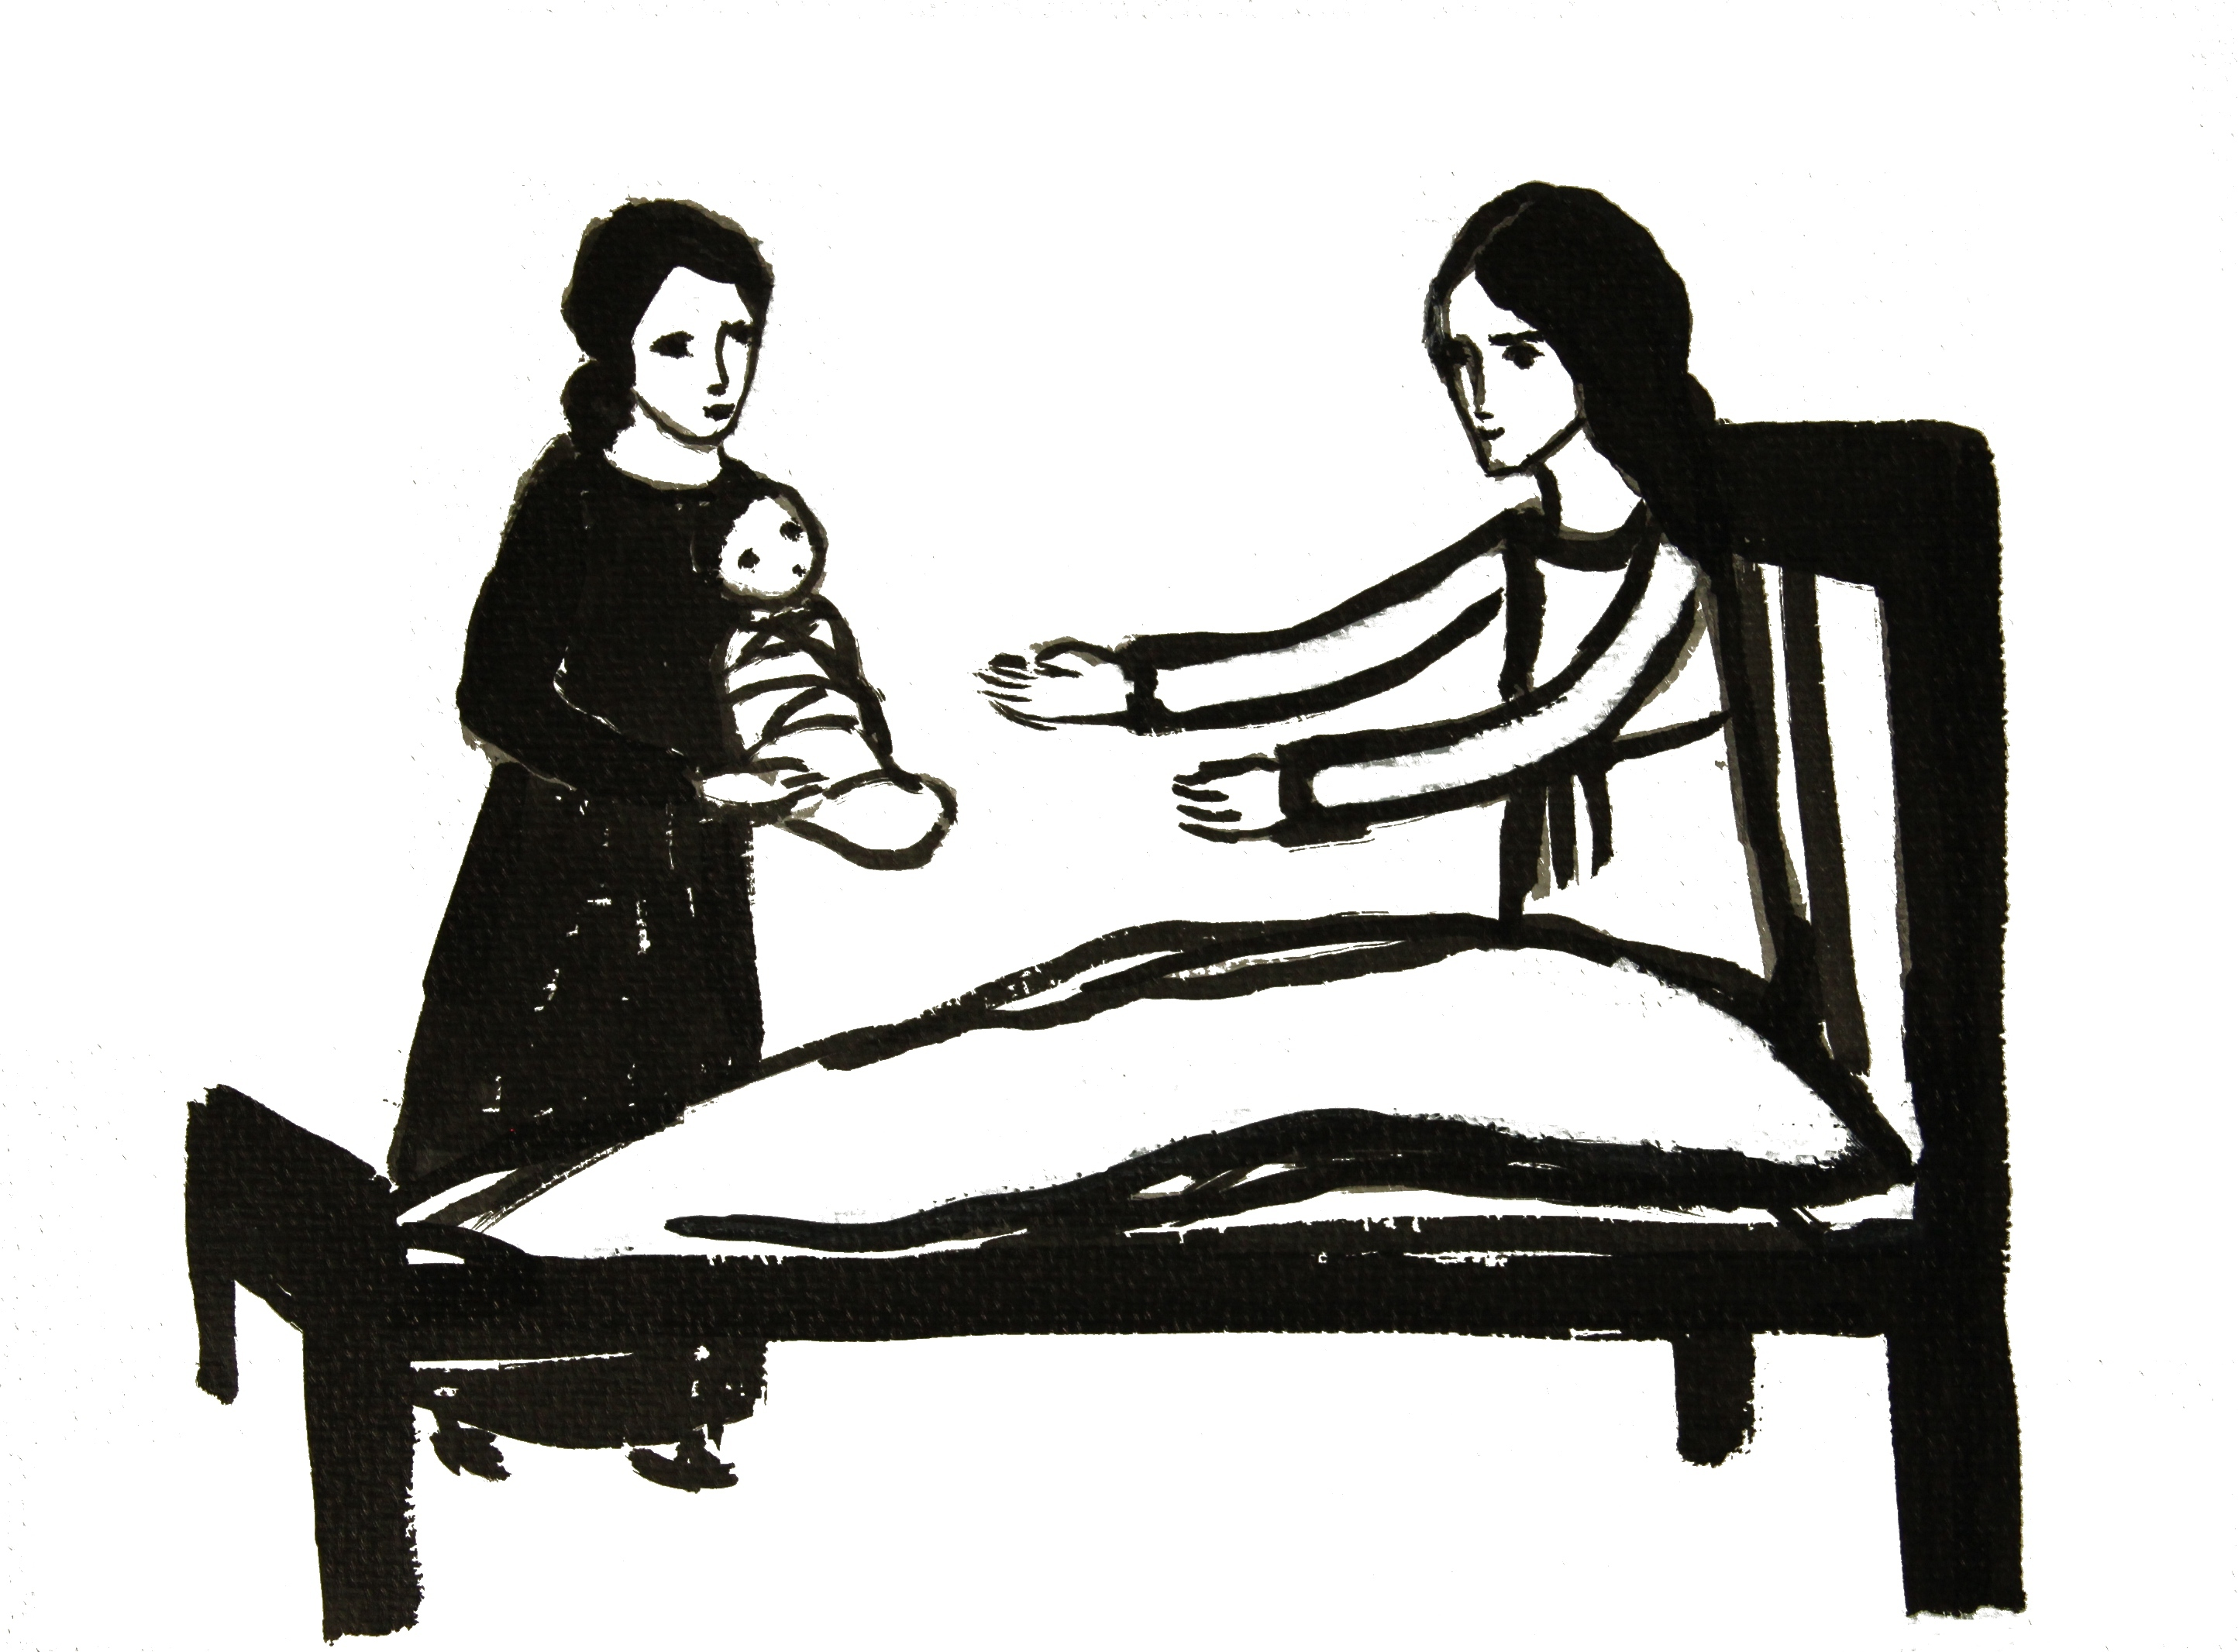
\includegraphics[width=10cm]{imagines/imago_nativitas.jpg}
\end{center}

\vfill

\begin{center}
Ad usum et secundum consuetudines chori \guillemotright Conventus Choralis\guillemotleft.

Editio Sancti Wolfgangi \annusEditionis
\end{center}

\pagebreak

\renewcommand{\headrulewidth}{0pt} % no horiz. rule at the header
\fancyhf{}
\pagestyle{fancy}

\pars{Oratio ante divinum Officium.}

\lettrine{{\color{red}A}}{peri,} Dómine, os meum ad benedicéndum nomen sanctum tuum:
munda quoque cor meum ab ómnibus vanis, pervérsis, et aliénis
cogitatiónibus:
intelléctum illúmina, afféctum inflámma,
ut digne, atténte ac devóte hoc Offícium recitáre váleam,
et exaudíri mérear ante conspéctum Divínæ Maiestátis tuæ.
Per Christum, Dominum nostrum.
\Rbardot{} Amen.

Dómine, in unióne illíus divínæ intentiónis,
qua ipse in terris laudes Deo persolvísti,
has tibi Horas \rubricatum{(vel \textnormal{hanc tibi Horam})} persólvo.

\trOratioAnteOfficium

\vfill

\pars{Oratio post divinum Officium.}

\rubrica{
  Orationem sequentem devote post Officium recitantibus
  Leo Papa X. defectus, et culpas in eo persolvendo ex humana
  fragilitate contractas, indulsit, et dicitur flexis genibus.
}

\lettrine{{\color{red}S}}{acrosánctæ} et indivíduæ Trinitáti,
crucifíxi Dómini nostri Iesu Christi humanitáti,
beatíssimæ et gloriosíssimæ sempérque Vírginis Maríæ
fecúndæ integritáti, 
et ómnium Sanctórum universitáti
sit sempitérna laus, honor, virtus et glória
ab omni creatúra,
nobísque remíssio ómnium peccatórum,
per infiníta sǽcula sæculórum.
\Rbardot{} Amen.

\noindent \Vbardot{} Beáta víscera Maríæ Virginis, quæ portavérunt
ætérni Patris Fílium.\\
\Rbardot{} Et beáta úbera, quæ lactavérunt Christum Dominum.

\rubrica{Et dicitur secreto \textnormal{Pater noster.} et \textnormal{Ave María.}}

\trOratioPostOfficium

\vfill

\hora{In Vesperis.} %%%%%%%%%%%%%%%%%%%%%%%%%%%%%%%%%%%%%%%%%%%%%%%%%%%%%
\sideThumbs{Vesperæ}

\label{deusinadiutorium}
{
\grechangedim{interwordspacetext}{0.18 cm plus 0.15 cm minus 0.05 cm}{scalable}%
\gregorioscore{temporalia/deusinadiutorium-communis.gtex}
\grechangedim{interwordspacetext}{0.32 cm plus 0.15 cm minus 0.05 cm}{scalable}%
}

\vfill
\pagebreak

\cantusCumNeumis

\pars{Psalmus 1.} \scriptura{\textbf{H307}}

{
\grechangedim{interwordspacetext}{0.28 cm plus 0.15 cm minus 0.05 cm}{scalable}%
\antiphona{VIII G}{temporalia/ant1.gtex}
\grechangedim{interwordspacetext}{0.32 cm plus 0.15 cm minus 0.05 cm}{scalable}%
}

\trAntI

\scriptura{Ps. 109}

\gregorioscore{temporalia/ps109-initium-viii-G-auto.gtex}

\psalmusEtTranslatioT{temporalia/ps109-comb.tex}{10cm}

\vfill
\pagebreak

\pars{Psalmus 2.} \scriptura{\textbf{H307}}

\antiphona{VII c}{temporalia/ant2.gtex}

\trAntII

\scriptura{Ps. 112}

\gregorioscore{temporalia/ps112-initium-vii-c-auto.gtex}
\psalmusEtTranslatioT{temporalia/ps112-comb.tex}{10cm}

\vfill
\pagebreak

\pars{Psalmus 3.} \scriptura{\textbf{H307}}

{
\grechangedim{interwordspacetext}{0.14 cm plus 0.15 cm minus 0.05 cm}{scalable}%
\antiphona{VI F}{temporalia/ant3.gtex}
\grechangedim{interwordspacetext}{0.32 cm plus 0.15 cm minus 0.05 cm}{scalable}%
}

\trAntIII

\scriptura{Ps. 121}

\gregorioscore{temporalia/ps121-initium-vi-F-auto.gtex}
\psalmusEtTranslatioT{temporalia/ps121-comb.tex}{10cm}

\vfill
\pagebreak

\pars{Psalmus 4.} \scriptura{\textbf{H308}}

{
\grechangedim{interwordspacetext}{0.24 cm plus 0.15 cm minus 0.05 cm}{scalable}%
\antiphona{VIII G}{temporalia/ant4.gtex}
\grechangedim{interwordspacetext}{0.32 cm plus 0.15 cm minus 0.05 cm}{scalable}%
}

\trAntIV

\scriptura{Ps. 126}

\gregorioscore{temporalia/ps126-initium-viii-G-auto.gtex}
\psalmusEtTranslatioT{temporalia/ps126-comb.tex}{10cm}

\vfill
\pagebreak

\raggedcolumns

% Capitulum. %%%
\cantusSineNeumas

\label{capitulum}
\pars{Capitulum.} \scriptura{Sir. 24, 14}

\gregorioscore{temporalia/capitulum-AbInitio.gtex}

% preklad Jeruz. bible
\trCapituli

\vfill
\pars{Responsorium breve.}

\antiphona{VI}{temporalia/resp1v.gtex}

\trRespVesp

\vfill
\pagebreak

% Hymnus. %%%
\pars{Hymnus.}

\superInitialam{I}
{
\grechangedim{interwordspacetext}{0.20 cm plus 0.15 cm minus 0.05 cm}{scalable}%
\gregorioscore{temporalia/hym-AveMarisStella.gtex}
\grechangedim{interwordspacetext}{0.32 cm plus 0.15 cm minus 0.05 cm}{scalable}%
}
{
\vspace{-0.3cm}
\setlength{\columnsep}{7pt} % prostor mezi sloupci
\begin{translatioMulticol}{3}
Zdrávas, hvězdo mořská, životodárná Matko Boží\\
a vždy Panno, šťastná nebes bráno.\\
\\
Přijímajíc ono Ave z Gabrielových úst,\\
upevni nás v pokoji, měníc jméno Evy.\\
\textit{(Slovní hříčka Ave - Eva.)}\columnbreak

Rozvaž pouta vinným, dej světlo slepým:\\
odežeň, co je na nás špatného, vypros všechno dobré.\\
\\
Ukaž, že jsi matka: skrze tebe ať přijme (naše) prosby\\
ten, jenž, když se pro nás narodil, přijal i to, že bude tvůj.\\
\\
Jedinečná Panno, mezi všemi mírná,\\
zbav nás našich hříchů, učiň mírnými a čistými.\columnbreak

Dej nám čistý život, připrav nám svou cestu:\\
abychom viděli Ježíše a vždy se s tebou radovali.\\
\\
Buď chvála Bohu Otci, nejvyššímu Kristu důs\-toj\-nost,\\
(tak i) Duchu Svatému; Třem jediná pocta.\\
Amen.
\end{translatioMulticol}

\setlength{\columnsep}{30pt} % prostor mezi sloupci
}

\pars{Versus.}

% Versus. %%%
\gregorioscore{temporalia/versus-nativitasest.gtex}
    
\noindent \trVersus

\vfill
\pagebreak

\cantusCumNeumis

\pars{Canticum B. Mariæ V.}\rubrica{ - in I. vesperis:}
\vspace{-0.5cm}

\antiphona{I D2}{temporalia/ant-magn-vesp1.gtex}

\trAntMagnificatI

\scriptura{Lc. 1, 46-55}

\cantusSineNeumas
\gregorioscore{temporalia/magnificat-initium-i-D2.gtex}

\vspace{-0.4cm}

\psalmusEtTranslatioT{temporalia/magnificat-comb.tex}{10.3cm}

\vfill
\pagebreak

\pars{Canticum B. Mariæ V.}\rubrica{ - in II. vesperis:} \scriptura{\textbf{H308}}
\label{magnificatIIvesp}

\cantusCumNeumis
\antiphona{I f}{temporalia/ant-magn-vesp2.gtex}

\trAntMagnificatII

\scriptura{Lc. 1, 46-55}

\cantusSineNeumas
\gregorioscore{temporalia/magnificat-initium-i-f.gtex}

%% maly svindl, ale prizvukova struktura Isoll-D2 a Isoll-f je stejna
\psalmusEtTranslatioT{temporalia/magnificat-comb.tex}{10.3cm}

\antiphona{}{temporalia/ant-magn-vesp2.gtex}

\vfill
\pagebreak

\label{oratio}
\anteOrationem

\pagebreak

%% Oratio. %%%
\pars{Oratio.}

\gregorioscore{temporalia/oratio.gtex}
\trOrationis

\vspace{1cm}
\rubrica{Hebdomadarius dicit iterum Dominus vobiscum. Postea cantatur a cantore:}
\vspace{2mm}

\gregorioscore{temporalia/benedicamus-duplex-vesperae.gtex}

\vfill
\pagebreak

\hora{Ad Completorium.} %%%%%%%%%%%%%%%%%%%%%%%%%%%%%%%%%%%%%%%%%%%%%%%%%%%%%%%%%%
\sideThumbs{{\scriptsize{}Completorium}}

\rubrica{Lector petit benedictionem, dicens:}

\gregorioscore{temporalia/jubedomnebenedicere.gtex}

\trJubeDomne

\vfill

\pars{Benedictio.}

\gregorioscore{temporalia/benedictio-noctemquietam.gtex}

\trComplBenedictio

\vfill

\pars{Lectio brevis.} \scriptura{1Ptr. 5, 8-9}

\gregorioscore{temporalia/lectiobrevis-fratressobrii.gtex}

\trComplLectioBr

\vfill

\noindent \Vbardot{} Adiutórium nostrum in nómine Dómini. \Rbardot{} Qui fecit cælum, et terram.

\vfill

\noindent Pater noster \rubricatum{quod dicitur totum secreto.}

\vfill
\pagebreak

\pars{Confessio.}

\noindent Confíteor Deo omnipoténti, beátæ Maríæ semper Vírgini, beáto
Michaéli Archángelo, beáto Ioánni Baptístæ, sanctis Apóstolis Petro
et Paulo, ómnibus Sanctis, et vobis fratres: quia peccávi nimis cogitatióne,
verbo et ópere: mea culpa, mea culpa, mea máxima culpa.
Ídeo precor beátam Maríam semper Vírginem, beátum Michaélum
Archángelum, beátum Ioánnem Baptístam, sanctos Apóstolos Petrum
et Paulum, omnes Sanctos, et vos fratres, oráre pro me ad Dóminum
Deum nostrum.

\vfill

\noindent \Vbardot{} Misereátur nostri omnípotens Deus, et, dimíssis peccátis nostris, perdúcat
nos ad vitam ætérnam. \Rbardot{} Amen.

\vfill

\noindent \Vbardot{} Indulgéntiam, absolutiónem et remissiónem peccatórum nostrórum tríbuat nobis
omnípotens et miséricors Dóminus. \Rbardot{} Amen.

\vfill

\rubrica{Et facta absolutione dicitur:}

\gregorioscore{temporalia/convertenosdeus.gtex}

\vfill

\gregorioscore{temporalia/deusinadiutorium-communis.gtex}

\vfill
\pagebreak

\pars{Psalmus 1.} \scriptura{Cf. Ps. 4, 2}

\antiphona{VIII G}{temporalia/ant-miserere.gtex}

\trComplAntI

\scriptura{Ps. 4}

\gregorioscore{temporalia/ps4-initium-viii-G-auto.gtex}

\psalmusEtTranslatioT{temporalia/ps4-comb.tex}{10cm}

\vfill
\pagebreak

\pars{Psalmus 2.} \scriptura{Ps. 90}

\psalmusEtTranslatioT{temporalia/ps90-comb.tex}{10cm}

\pagebreak

\pars{Psalmus 3.} \scriptura{Ps. 133}

\psalmusEtTranslatioT{temporalia/ps133-comb.tex}{10cm}

\vfill

\antiphona{}{temporalia/ant-miserere.gtex}

\vfill

\pars{Hymnus.}

\antiphona{II}{temporalia/hym-TeLucis.gtex}
\begin{translatioMulticol}{3}
Než světlo zhasne prosíme\\
Tebe tvůrce všech pokorně,\\
abys nám ve své milosti\\
byl ochranou a~pomocí.\columnbreak

Ať vzdáleny jsou od nás sny\\
a~těžké noční přízraky.\\
Zdrť našeho nepřítele,\\
těla poskvrn ať ujdeme.\columnbreak

Tobě buď sláva, Ježíši,\\
národům že ses projevil,\\
Otci i~Duchu života\\
po věkoucí věky světa.\\
Amen.
\end{translatioMulticol}


\pagebreak

\pars{Capitulum.} \scriptura{Ier. 14, 9}

\gregorioscore{temporalia/capitulum-tuautem.gtex}

% preklad Jeruz. bible
\trComplCapituli

\vfill

\pars{Responsorium breve.} \scriptura{Ps. 30, 6}

\superInitialam{VI}
\gregorioscore{temporalia/resp-inmanus.gtex}

\trRespCompl
\vfill

\pars{Versus.} \scriptura{Ps. 16, 8}

{
\grechangedim{interwordspacetext}{0.24 cm plus 0.15 cm minus 0.05 cm}{scalable}%
\gregorioscore{temporalia/versus-custodi.gtex}
\grechangedim{interwordspacetext}{0.32 cm plus 0.15 cm minus 0.05 cm}{scalable}%
}

\noindent \trComplVersus

\vfill
\pagebreak

\cantusCumNeumis

\pars{Canticum Simeonis.}

{
\grechangedim{interwordspacetext}{0.30 cm plus 0.15 cm minus 0.05 cm}{scalable}%
\antiphona{III a}{temporalia/ant-salvanos-antiquo.gtex}
\grechangedim{interwordspacetext}{0.32 cm plus 0.15 cm minus 0.05 cm}{scalable}%
}

\trAntSalvaNos

\scriptura{Lc. 2, 29-32}

\gregorioscore{temporalia/nuncdimittis-initium-iii-a-auto.gtex}

\psalmusEtTranslatioT{temporalia/nuncdimittis-comb.tex}{10cm}

\vfill
\pagebreak

\pars{Oratio.}

\cantusSineNeumas

\gregorioscore{temporalia/oratio-visita.gtex}

\trComplOrationis

\vfill

\gregorioscore{temporalia/domineexaudi.gtex}

\vfill

\gregorioscore{temporalia/benedicamus-minor.gtex}

\vfill

\pars{Benedictio.}

\noindent Benedícat et custódiat nos omnípotens et miséricors Dóminus, \gredagger{}
Pater, et Fílius, et Spíritus Sanctus. \Rbardot{} Amen.

\vfill
\pagebreak

\pars{Antiphona finalis B. M. V.}

\antiphona{V}{temporalia/ant-salveregina-simplex.gtex}

\trSalveRegina

\vspace{0.5cm}

\gregorioscore{temporalia/versus-orapronobis.gtex}

\trOraProNobis

\vfill
\pagebreak

\hora{Ad Matutinum.} %%%%%%%%%%%%%%%%%%%%%%%%%%%%%%%%%%%%%%%%%%%%%%%%%%%%%%%%%%
\sideThumbs{Matutinum}

\vspace{2mm}

\gregorioscore{temporalia/dominelabiamea.gtex}

\vspace{2mm}

\pars{Invitatorium.}

\vspace{-2mm}

\antiphona{V}{temporalia/matinv-NativitatemVirginis.gtex}

\trMatInvitatorium

\scriptura{Ps. 94 (Textus antiquus latinus); \textbf{H449}}

\vspace{-5mm}

\antiphona{II}{temporalia/venite2a.gtex}

\trMatVeniteA

\scriptura{Repetitur integrum Invitatorium.}

\antiphona{}{temporalia/venite2b.gtex}

\trMatVeniteB

\scriptura{Repetitur altera pars Invitatorii.}

\rubrica{In sequenti Psalmi versu, ad verba \textnormal{veníte, adorémus et procidámus ante Deum}, genuflectitur.}

\antiphona{}{temporalia/venite2c.gtex}

\trMatVeniteC

\scriptura{Repetitur integrum Invitatorium.}

\antiphona{}{temporalia/venite2d.gtex}

\trMatVeniteD

\scriptura{Repetitur altera pars Invitatorii.}

\vfill
\pagebreak

\antiphona{}{temporalia/venite2e.gtex}

\trMatVeniteE

\scriptura{Repetitur integrum Invitatorium.}

\antiphona{}{temporalia/venite2f.gtex}

\scriptura{Repetitur altera pars Invitatorii. Denique repetitur integrum Invitatorium.}

\antiphona{}{temporalia/matinv-NativitatemVirginis.gtex}

\vfill
\pagebreak

\pars{Hymnus.}

\vspace{-0.5cm}

{
\grechangedim{interwordspacetext}{0.30 cm plus 0.15 cm minus 0.05 cm}{scalable}%
\antiphona{II}{temporalia/hym-QuemTerra.gtex}
\grechangedim{interwordspacetext}{0.32 cm plus 0.15 cm minus 0.05 cm}{scalable}%
}
{
\vspace{0.5cm}
\setlength{\columnsep}{0pt} % prostor mezi sloupci
\begin{translatioMulticol}{5}
Jenž vzýván zemí, hvězdami\\
i mořem uctívaný,\\
jenž trojím vládne ústrojím,\\
toho Mariin nosí klín.\columnbreak

A jemuž slunce, měsíc, vše\\
svým čase službu skýtají,\\
toho z nebeské milosti\\
dívčiny hostí útroby.\columnbreak

Matko blažená útěžkem,\\
vždyť Tvůrce nad vše velkého,\\
jenž v špetce hrsti třímá svět\\
nitru tvému smí náležet.\columnbreak

Nebeským poslem slavená\\
Svatým Duchm obtížená,\\
na svět z jeskyně vyšel z ní,\\
na nějž národy čekají.\columnbreak

Na věky  ti Kriste sláva,\\
Ježíši z Panny zrozený,\\
s Otcem a Duchem blaženým\\
buď národy zvěstována.
Amen.
\end{translatioMulticol}

\setlength{\columnsep}{30pt} % prostor mezi sloupci
}

\vfill
\pagebreak

\subhora{In I. Nocturno}

\pars{Psalmus 1.} \scriptura{Lc. 1, 42; \textbf{H21}}

\antiphona{IV A}{temporalia/matant1.gtex}

\trMatAntI

\scriptura{Psalmus 8.}

\gregorioscore{temporalia/ps8-initium-iv-A-auto.gtex}

\psalmusEtTranslatioT{temporalia/ps8-comb.tex}{10cm}

%\antiphona{}{temporalia/matant1.gtex} % repeat the antiphon - new page

\vfill
\pagebreak

\pars{Psalmus 2.} \scriptura{Cf. Sir. 24, 20; \textbf{H115}}

\antiphona{IV A}{temporalia/matant2.gtex}

\trMatAntII

\scriptura{Psalmus 18.}

\gregorioscore{temporalia/ps18-initium-iv-A-auto.gtex}

\psalmusEtTranslatioT{temporalia/ps18-comb.tex}{10cm}

\antiphona{}{temporalia/matant2.gtex} % repeat the antiphon - new page

\vfill
\pagebreak

\pars{Psalmus 3.} \scriptura{\textbf{H115}}

\antiphona{IV A}{temporalia/matant3.gtex}

\trMatAntIII

\scriptura{Psalmus 23.}

\gregorioscore{temporalia/ps23-initium-iv-A-auto.gtex}

\psalmusEtTranslatioT{temporalia/ps23-comb.tex}{10cm}

\vfill
\pagebreak

\pars{Versus.} \scriptura{Ps. 44, 5}

\gregorioscore{temporalia/versus-specie.gtex}

\noindent \trMatVersusI

\vfill

\gregorioscore{temporalia/oratiodominica-mat.gtex}

\vfill

\pars{Absolutio.}

\gregorioscore{temporalia/absolutio-exaudi.gtex}

\trMatAbsolutioI

\vfill
\pagebreak

\gregorioscore{temporalia/benedictio-solemn-benedictione.gtex}

\trMatBenedictioI

\vfill

\gregorioscore{temporalia/tonus-lectionis-solemnis.gtex}

\vfill

\pars{Lectio I.} \scriptura{Ct. 1, 1-4}

\noindent Incípiunt Cántica canti\textit{có}rum.

\textusEtTranslatio{
  Osculétur me oscúlo oris sui; quia melióra sunt úbera tua vino,
  Fragrántia unguentis óptimis. Oleum effúsum nomen tuum;
  ídeo adolescéntulæ dilexérunt te.
  Trahe me, post te currémus in odórem unguentórum tuórum.
  Introdúxit me Rex in cellária sua;
  exsultábimus et lætábimur in te, memóres úberum tuórum super vinum.
  Recti díligunt te.
  Nigra sum, sed formósa, fíliæ Ierúsalem, sicut tabernácula Cedar,
  sicut pelles Salomónis.
}{\trMatLecI}{10cm}

\tuAutem

\vfill
\pagebreak

\pars{Responsorium 1.} \scriptura{\textbf{H305}}

\responsorium{III}{temporalia/matresp1.gtex}{\trMatRespI}

\vfill
\pagebreak

\gregorioscore{temporalia/benedictio-solemn-unigenitus.gtex}

\trMatBenedictioII

\vfill

\pars{Lectio II.} \scriptura{Ct. 1, 5-9}

\textusEtTranslatio{
  Nolíte me consideráre quod fusca sim, quia decolorávit me sol.
  Fílii matris meæ pugnavérunt contra me; posuérunt me custódem in víneis:
  víneam meam non custodívi.
  Indica mihi, quem díligit ánima mea, ubi pascas, ubi cubes in merídie,
  ne vagári incípiam post greges sodálium tuórum.
  Si ignóras te, o pulchérrima inter mulíeres, egrédere,
  et abi post vestígia gregum, et pasce hædos tuos iuxta tabernácula pastórum.
  Equitátui meo in cúrribus Pharaónis assimilávi te, amíca mea.
  Pulchræ sunt genæ tuæ sicut túrturis; collum tuum sicut monília.
}{\trMatLecII}{10cm}

\tuAutem

\vfill
\pagebreak

\pars{Responsorium 2.} \scriptura{\textbf{H305}}

\responsorium{IV}{temporalia/matresp2.gtex}{\trMatRespII}

\vfill
\pagebreak

\gregorioscore{temporalia/benedictio-solemn-spiritus.gtex}

\trMatBenedictioIII

\vfill

\pars{Lectio III.} \scriptura{Ct. 1, 10-16}

\textusEtTranslatio{
  Murénulas áureas faciémus tibi, vermiculátas argénto.
  Dum esset Rex in accúbitu suo, nardus mea dedit odórem suum.
  Fascículus myrrhæ diléctus meus mihi; inter úbera mea commorábitur.
  Botrus cypri diléctus meus mihi in víneis Engaddi.
  Ecce tu pulchra es, amíca mea; ecce tu pulchra es; óculi tui columbárum.
  Ecce tu pulcher es, dilécte mi, et decórus! Léctulus noster flóridus,
  Tigna domórum nostrárum cédrina, laqueária nostra cypréssina.
}{\trMatLecIII}{10cm}

\tuAutem

\vfill
\pagebreak

\pars{Responsorium 3.} \scriptura{\textbf{H305}}

\responsorium{II}{temporalia/matresp3.gtex}{\trMatRespIII}

\vfill
\pagebreak

\subhora{In II. Nocturno}

\pars{Psalmus 4.} \scriptura{Ps. 44, 5; \textbf{H117}}

\antiphona{VII c}{temporalia/matant4.gtex}

\trMatAntIV

\scriptura{Psalmus 44.}

\gregorioscore{temporalia/ps44-initium-vii-c-auto.gtex}

\psalmusEtTranslatioT{temporalia/ps44-comb.tex}{10cm}

\antiphona{}{temporalia/matant4.gtex} % repeat the antiphon - new page

\vfill
\pagebreak

\pars{Psalmus 5.} \scriptura{Ps. 45, 6; \textbf{H117}}

\antiphona{VII c}{temporalia/matant5.gtex}

\trMatAntV

\scriptura{Psalmus 45.}

\gregorioscore{temporalia/ps45-initium-vii-c-auto.gtex}

\psalmusEtTranslatioT{temporalia/ps45-comb.tex}{10cm}

%\antiphona{}{temporalia/matant5.gtex} % repeat the antiphon - new page

\vfill
\pagebreak

\pars{Psalmus 6.} \scriptura{Psalmus 86, 7; \textbf{H117}}

\antiphona{VII c}{temporalia/matant6.gtex}

\trMatAntVI

\scriptura{Psalmus 86.}

\gregorioscore{temporalia/ps86-initium-vii-c-auto.gtex}

\psalmusEtTranslatioT{temporalia/ps86-comb.tex}{10cm}

%\antiphona{}{temporalia/matant6.gtex} % repeat the antiphon - new page

\vfill
\pagebreak

\pars{Versus.}

\gregorioscore{temporalia/versus-adjuvabit.gtex}

\noindent \trMatVersusII

\vfill

\gregorioscore{temporalia/oratiodominica-mat.gtex}

\vfill

\pars{Absolutio.}

\gregorioscore{temporalia/absolutio-ipsius.gtex}

\trMatAbsolutioII

\vfill
\pagebreak

\gregorioscore{temporalia/benedictio-solemn-deus.gtex}

\trMatBenedictioIV

\vfill

% Sermo sancti Augustíni Epíscopi.
\pars{Lectio IV.} \scriptura{Sermo 18. de Sanctis, qui est II. de Annut. Dominica.}

\noindent Sermo sancti Augustíni \textit{E}píscopi.

\textusEtTranslatio{
  Adest nobis, dilectíssimi, optátus dies beátæ ac venerábilis semper
  Vírginis Maríæ: ídeo cum summa exsultatióne gáudeat terra nostra, tantæ
  Vírginis illustráta natáli. Hæc est enim flos campi, de qua ortum est
  pretiósum lílium convállium, per cuius partum mutátur natúra protoplastórum,
  delétur et culpa. Præcísum est in ea illud Hevae infelicitátis elógium, quo
  dícitur: In dolóre páries fílios tuos; quia ista in lætítia Dóminum péperit.
}{\trMatLecIV}{10cm}

\tuAutem

\vfill
\pagebreak

\pars{Responsorium 4.} \scriptura{\textbf{H306}}

\responsorium{I}{temporalia/matresp4.gtex}{\trMatRespIV}

\vfill
\pagebreak

\gregorioscore{temporalia/benedictio-solemn-christus.gtex}

\trMatBenedictioV

\vfill

\pars{Lectio V.} \scriptura{Sermo 18. de Sanctis, qui est II. de Annut. Dominica.}

\textusEtTranslatio{
  Heva enim luxit, ista exsultávit: Heva lácrimas,
  María gáudium in ventre portávit: quia illa peccatórem, ista édidit innocéntem.
  Mater géneris nostri pœnam íntulit mundo, Génitrix Dómini nostri salútem íntulit mundo.
  Auctrix peccáti Heva, auctrix mériti María.
  Heva occídendo óbfuit, María vivificándo prófuit.
  Illa percússit, ista sanávit.
  Pro inobediéntia enim obediéntia commutátur, fides pro perfídia compensátur.
}{\trMatLecV}{10cm}

\tuAutem

\vfill
\pagebreak

\pars{Responsorium 5.}

\responsorium{VIII}{temporalia/matresp5.gtex}{\trMatRespV}

\vfill
\pagebreak

\gregorioscore{temporalia/benedictio-solemn-ignem.gtex}

\trMatBenedictioVI

\vfill

\pars{Lectio VI.} \scriptura{Sermo 18. de Sanctis, qui est II. de Annut. Dominica.}

\textusEtTranslatio{
  Plaudat nunc órganis María, et inter velóces artículos tympána puerpéræ concrépent.
  Concínant lætántes chori, et alternántibus módulis dulcisóna carmína misceántur.
  Audíte ígitur quemádmodum tympanistría nostra cantáverit.
  Ait enim: Magníficat ánima mea Dóminum: et exsultávit spíritus meus in Deo   salutári meo.
  Quia respéxit humilitátem ancíllæ suæ: ecce enim ex hoc beátam me dícent omnes generatiónes.
  Quia fecit mihi magna qui potens est.
  Causam ígitur invalescéntis errati miráculum novi partus evícit, et Hevae planctum Maríæ cantus exclúsit.
}{\trMatLecVI}{10cm}

\tuAutem

\vfill
\pagebreak

\pars{Responsorium 6.} \scriptura{\Rbar{} Cantor \Vbar{} Lc. 1, 42; \textbf{H307}}

\responsorium{I}{temporalia/matresp6.gtex}{\trMatRespVI}

\vfill
\pagebreak

\subhora{In III. Nocturno}

\pars{Psalmus 7.} \scriptura{\textbf{H117}}

\vspace{-0.2cm}

\antiphona{IV c}{temporalia/matant7.gtex}

\trMatAntVII

\scriptura{Psalmus 95.}

\gregorioscore{temporalia/ps95-initium-iv-c-auto.gtex}

\psalmusEtTranslatioT{temporalia/ps95-comb.tex}{10.5cm}

\antiphona{}{temporalia/matant7.gtex} % repeat the antiphon - new page

\vfill
\pagebreak

\pars{Psalmus 8.} \scriptura{\textbf{H117}}

\antiphona{IV c}{temporalia/matant8.gtex}

\trMatAntVIII

\scriptura{Psalmus 96.}

\gregorioscore{temporalia/ps96-initium-iv-c-auto.gtex}

\psalmusEtTranslatioT{temporalia/ps96-comb.tex}{10cm}

%\antiphona{}{temporalia/matant8.gtex} % repeat the antiphon - new page

\vfill
\pagebreak

\pars{Psalmus 9.} \scriptura{\textbf{H116}}

\antiphona{IV c}{temporalia/matant9.gtex}

\trMatAntIX

\scriptura{Psalmus 97.}

\gregorioscore{temporalia/ps97-initium-iv-c-auto.gtex}

\psalmusEtTranslatioT{temporalia/ps97-comb.tex}{10cm}

\vfill
\pagebreak

\pars{Versus.}

\gregorioscore{temporalia/versus-elegit.gtex}

\noindent \trMatVersusIII

\vfill

\gregorioscore{temporalia/oratiodominica-mat.gtex}

\vfill

\pars{Absolutio.}

\gregorioscore{temporalia/absolutio-avinculis.gtex}

\trMatAbsolutioIII

\vfill
\pagebreak

\gregorioscore{temporalia/benedictio-solemn-evangelica.gtex}

\trMatBenedictioVII

\vfill

% Léctio sancti Evangélii secúndum Matthǽum.
\pars{Lectio VII.} \scriptura{Mt. 1, 1-16}

\noindent Léctio sancti Evangélii secúndum \textit{Mat}thǽum.

\textusEtTranslatio{
  Liber generatiónis Iesu Christi, fílii David, fílii Abraham.
  Abraham génuit Isaac.
  Isaac autem génuit Iacob.
  \textit{Et} réliqua.
}{\trMatLecVIIa}{10cm}

% Homilía sancti Hieronymi Presbyteri.
\scriptura{Lib. 1. Comm. in Matth., in initio.}

\noindent Homilía sancti Hierónymi \textit{Pres}býteri.

\textusEtTranslatio{
  In Isaía légimus: Generatiónem eius quis enarrábit?
  Non ergo putémus Evangelístam Prophétæ esse contrárium,
  ut quod ille impossíbile dixit effátu, hic narráre incípiat:
  quia ibi de generatióne divinitátis, hic de incarnatióne est dictum.
  A carnálibus autem cœpit, ut per hóminem, Deum díscere incipiámus.
  Fílii David, fílii Abraham. Ordo præpósterus, sed necessário commutátus.
  Si enim primum posuísset Abraham, et póstea David,
  rursus ei repeténdus fúerat Abraham, ut generatiónis séries texerétur.
}{\trMatLecVIIb}{10cm}

\tuAutem

\vfill
\pagebreak

\pars{Responsorium 7.} \scriptura{\Rbar{} Lc. 1, 48 \Vbar{} ibid. 1, 50; \textbf{H297}}

\responsorium{VIII}{temporalia/matresp7.gtex}{\trMatRespVII}

\vfill
\pagebreak

\gregorioscore{temporalia/benedictio-solemn-cujus.gtex}

\trMatBenedictioVIII

\vfill

\pars{Lectio VIII.} \scriptura{Lib. 1. Comm. in Matth., in initio.}

\textusEtTranslatio{
  Ideo autem céteris prætermíssis, horum fílium nuncupávit:
  quia ad hos tantum facta est de Christo repromíssio.
  Ad Abraham: In sémine, inquit, tuo benedicéntur omnes gentes:
  quod est Christus.
  Ad David: De fructu ventris tui ponam super sedem tuam.
  Iudas autem génuit Phares et Zaram de Thamar.
  Notándum, in genealogía Salvatóris nullam sanctárum assúmi mulíerum,
  sed eas quas Scriptúra reprehéndit: ut qui propter peccatóres vénerat,
  de peccatóribus nascens, ómnium peccáta deléret.
  Unde et in consequéntibus Ruth Moabítis pónitur, et Bethsabée uxor Uríæ.
}{\trMatLecVIII}{10cm}

\tuAutem

\vfill
\pagebreak

\pars{Responsorium 8.} \scriptura{\Rbar{} Cf. Mal. 4, 2 \Vbar{} S. Augustini sermo 18 de Sanctis; \textbf{H307}}

\responsorium{I}{temporalia/matresp8.gtex}{\trMatRespVIII}

\vfill
\pagebreak

\gregorioscore{temporalia/benedictio-solemn-adsocietatem.gtex}

\trMatBenedictioIX

\vfill

\pars{Lectio IX.} \scriptura{Lib. 1. Comm. in Matth., in initio.}

\textusEtTranslatio{
  Quínimmo beáti qui áudiunt verbum Dei, et custódiunt.
  Pulchre Salvátor attestatióni mulíeris ánnuit,
  non eam tantúmmodo quæ Verbum Dei corporáliter generáre merúerat,
  sed et omnes qui idem Verbum spiritáliter audítu fídei concípere,
  et boni óperis custódia vel in suo, vel in proximórum corde párere,
  et quasi álere studúerint, assevérans esse beátos: quia et éadem Dei Génitrix,
  et inde quidem beáta, quia Verbi incarnándi minístra facta est temporális;
  sed inde multo beátior, quia eiúsdem semper amándi custos, manébat ætérna.
}{\trMatLecIX}{10cm}

\tuAutem

\vfill
\pagebreak

% Te Deum

\pars{Hymnus Ambrosianus}

\superInitialam{III}
\gregorioscore{temporalia/tedeum-solemnis.gtex}

\trTeDeum

\vfill
\pagebreak

% Evangelium

\gregorioscore{temporalia/tonus-evangelii-b.gtex}

\vfill

\pars{Léctio san\textit{cti} Evangélii {\textnormal{\grestar{}}} secúndum Mat\textit{thǽ}um.} \scriptura{Matth. 1, 1-16}

\textusEtTranslatio{
  Liber generatiónis Iesu Christi, fílii David, fílii Abraham.
  Abraham génuit Isaac.
  Isaac autem génuit Iacob.
  Iacob autem génuit Iudam et fratres eius.
  Iudas autem génuit Phares et Zaram de Thamar.
  Phares autem génuit Esron.
  Esron autem génuit Aram.
  Aram autem génuit Amínabad.
  Amínabad autem génuit Naásson.
  Naásson autem génuit Salmon.
  Salmon autem génuit Booz de Rahab.
  Booz autem génuit Obed ex Ruth.
  Obed autem génuit Iesse.
  Iesse autem génuit David regem.
  David autem rex génuit Salomónem ex ea, quæ fuit Uríæ.
  Sálomon autem génuit Róboam.
  Róboam autem génuit Abíam.
  Abías autem génuit Asa.
  Asa autem génuit Iósaphat.
  Iósaphat autem génuit Ioram.
  Ioram autem génuit Ozíam.
  Ozías autem génuit Ióatham.
  Ióatham autem génuit Achaz.
  Achaz autem génuit Ezechíam.
  Ezechías autem génuit Manássen.
  Manásses autem génuit Amon.
  Amon autem génuit Iosíam.
  Iosías autem génuit Iechoníam et fratres eius in transmigratióne Babylónis.
  Et post transmigratiónem Babylónis: Iechonías génuit Saláthiel.
  Saláthiel autem génuit Zoróbabel.
  Zoróbabel autem génuit Abiud.
  Abiud autem génuit Elíacim.
  Elíacim autem génuit Azor.
  Azor autem génuit Sadoc.
  Sadoc autem génuit Achim.
  Achim autem génuit Eliud.
  Eliud autem génuit Eleázar.
  Eleázar autem génuit Mathan.
  Mathan autem génuit Iacob.
  Iacob autem génuit Ioseph, virum Maríæ, de qua natus est Iesus, qui vocátur Christus.
}{\trMatEvangelium}{10cm}

\vfill
\superInitialam{I}
\gregorioscore{temporalia/tedecetlaus.gtex}

\trTeDecetLaus

\vfill
\pagebreak

\gregorioscore{temporalia/domineexaudi.gtex}

\vfill

\pars{Oratio.}

\gregorioscore{temporalia/oratio.gtex}
\trOrationis

\vfill

\noindent \Vbardot{} Dómine, exáudi oratiónem meam.
\Rbardot{} Et clamor meus ad te véniat.

\vfill

% Nocturnale Romanum 2002, p. LXXVI Benedicamus Domino seems to match
% the one from Solemn Laudes.
\gregorioscore{temporalia/benedicamus-solemnis-laud.gtex}

\vfill

\noindent \Vbardot{} Fidélium ánimæ per misericórdiam Dei requiéscant in pace.
\Rbardot{} Amen.

\trFideliumAnimae

\vfill
\pagebreak

\hora{Ad Tertiam.} %%%%%%%%%%%%%%%%%%%%%%%%%%%%%%%%%%%%%%%%%%%%%%%%%%%%%%%%%%
\sideThumbs{Tertia}

\vspace{1cm}
\gregorioscore{temporalia/deusinadiutorium-communis.gtex}
\vspace{1cm}

\pars{Hymnus.}

\superInitialam{II}
\gregorioscore{temporalia/hym-NuncSancte.gtex}
\begin{translatioMulticol}{3}
Nyní nás Duchu přesvatý\\
s Otcem a Synem pronikni,\\
v okamžik jediný do srdce\\
vstup a zal\ij{} je milostí.\columnbreak

Ať ústa, jazyk i smysly,\\
mysl a síla vyznají,\\
ať ohněm láska zaplane\\
horlivá ke všem bližním.\columnbreak

Tobě buď sláva, náš Pane,\\
národům že ses projevil,\\
Otci i Duchu života\\
po věkoucí věky světa.\\
Amen.
\end{translatioMulticol}


\vfill
\pagebreak

\pars{Psalmus.} \scriptura{\textbf{H307}}

\antiphona{VII c}{temporalia/ant2.gtex}

\trAntII

\scriptura{Ps. 118, 33-80}

\gregorioscore{temporalia/ps118v_vi-initium-vii-c-auto.gtex}

\psalmusEtTranslatioT{temporalia/ps118v_vi-comb.tex}{10cm}

\vspace{-0.5cm}

\psalmusEtTranslatioT{temporalia/ps118vii_viii-comb.tex}{10cm}

\vspace{-0.5cm}

\psalmusEtTranslatioT{temporalia/ps118ix_x-comb.tex}{10cm}

\vspace{-0.5cm}

\antiphona{}{temporalia/ant2.gtex} % repeat the antiphon - new page

\vfill
\pagebreak

\raggedcolumns

% Capitulum. %%%
\cantusSineNeumas

\pars{Capitulum.} \scriptura{Sir. 24, 14}

\gregorioscore{temporalia/capitulum-AbInitio.gtex}

% preklad Jeruz. bible
\trCapituli

\vfill

\pars{Versus.}

{
\grechangedim{interwordspacetext}{0.28 cm plus 0.15 cm minus 0.05 cm}{scalable}%
\gregorioscore{temporalia/versus-specie.gtex}
\grechangedim{interwordspacetext}{0.32 cm plus 0.15 cm minus 0.05 cm}{scalable}%
}

%\noindent \trVersusTertia

\vfill

\rubrica{Ante Orationem, cantatur a Superiore:}

\pars{Supplicatio Litaniæ.}

\gregorioscore{temporalia/supplicatiolitaniae.gtex}

\vfill

\pars{Oratio Dominica.}

\gregorioscore{temporalia/oratiodominica-mat.gtex}

\vfill

\gregorioscore{temporalia/domineexaudi.gtex}

\vfill
\pagebreak

% Oratio. %%%
\pars{Oratio.}

\gregorioscore{temporalia/oratio.gtex}
\trOrationis

\vfill

\gregorioscore{temporalia/benedicamus-minor.gtex}

\vfill

\noindent \Vbardot{} Fidélium ánimæ per misericórdiam Dei requiéscant in pace.
\Rbardot{} Amen.

\trFideliumAnimae

\vfill
\pagebreak

\hora{Ad Laudes.} %%%%%%%%%%%%%%%%%%%%%%%%%%%%%%%%%%%%%%%%%%%%%%%%%%%%%%%%%%
\sideThumbs{Laudes}

% Psalmi festivi (AM33, pg. 721):
% 66 // 92, 99, 62, Dan3, 148+149+150

\vspace{1cm}
\gregorioscore{temporalia/deusinadiutorium-communis.gtex}
\vspace{1cm}

\cantusSineNeumas

\pars{Psalmus 1.} \scriptura{Ps. 66}

{
\grechangedim{interwordspacetext}{0.28 cm plus 0.15 cm minus 0.05 cm}{scalable}%
\gregorioscore{temporalia/ps66-initium-dir-auto.gtex}
\grechangedim{interwordspacetext}{0.32 cm plus 0.15 cm minus 0.05 cm}{scalable}%
}

\psalmusEtTranslatioT{temporalia/ps66-comb.tex}{10cm}

\vfill
\pagebreak

\pars{Psalmus 2.} \scriptura{\textbf{H307}}

{
\grechangedim{interwordspacetext}{0.28 cm plus 0.15 cm minus 0.05 cm}{scalable}%
\antiphona{VIII G}{temporalia/ant1.gtex}
\grechangedim{interwordspacetext}{0.32 cm plus 0.15 cm minus 0.05 cm}{scalable}%
}

\trAntI

\scriptura{Ps. 92}

\gregorioscore{temporalia/ps92-initium-viii-G-auto.gtex}

\psalmusEtTranslatioT{temporalia/ps92-comb.tex}{10cm}

\vfill
\pagebreak

\pars{Psalmus 3.} \scriptura{\textbf{H307}}

\antiphona{VII c}{temporalia/ant2.gtex}

\trAntII

\scriptura{Ps. 99}

\gregorioscore{temporalia/ps99-initium-vii-c-auto.gtex}

\psalmusEtTranslatioT{temporalia/ps99-comb.tex}{10cm}

\vfill
\pagebreak

\pars{Psalmus 4.} \scriptura{\textbf{H307}}

\vspace{-0.3cm}

{
\grechangedim{interwordspacetext}{0.14 cm plus 0.15 cm minus 0.05 cm}{scalable}%
\antiphona{VI F}{temporalia/ant3.gtex}
\grechangedim{interwordspacetext}{0.32 cm plus 0.15 cm minus 0.05 cm}{scalable}%
}

\trAntIII

\scriptura{Ps. 62.}

\gregorioscore{temporalia/ps62-initium-vi-F-auto.gtex}

\vspace{-0.6cm}

\psalmusEtTranslatioT{temporalia/ps62-comb.tex}{10cm}

\vfill
\pagebreak

\pars{Psalmus 5.} \scriptura{\textbf{H308}}

{
\grechangedim{interwordspacetext}{0.24 cm plus 0.15 cm minus 0.05 cm}{scalable}%
\antiphona{VIII G}{temporalia/ant4.gtex}
\grechangedim{interwordspacetext}{0.32 cm plus 0.15 cm minus 0.05 cm}{scalable}%
}

\trAntIV

\scriptura{Canticum trium puerorum, Dan. 3, 57-88 et 56}

\gregorioscore{temporalia/dan3-initium-viii-G-auto.gtex}

\psalmusEtTranslatioT{temporalia/dan3-comb.tex}{10cm}

\rubrica{Hic non dicitur Gloria Patri, neque Amen.}
\vspace{1cm}

\gregorioscore{temporalia/ant4.gtex} % repeat the antiphon - new page

\vfill
\pagebreak

\pars{Psalmus 6.} \scriptura{\textbf{H308}}

{
\grechangedim{interwordspacetext}{0.14 cm plus 0.15 cm minus 0.05 cm}{scalable}%
\antiphona{VII c}{temporalia/ant5.gtex}
\grechangedim{interwordspacetext}{0.32 cm plus 0.15 cm minus 0.05 cm}{scalable}%
}

\trAntV

\scriptura{Ps. 148}

\gregorioscore{temporalia/ps148-initium-vii-c-auto.gtex}

\newlength{\psVItransW}
\setlength{\psVItransW}{10.5cm}

\psalmusEtTranslatioT{temporalia/ps148-comb.tex}{10cm}

\vspace{-0.5cm}

\rubrica{Hic non dicitur Gloria Patri.}

\vfill
\pagebreak

%
\scriptura{Ps. 149}

\gregorioscore{temporalia/ps149-initium-vii-c-auto.gtex}

\psalmusEtTranslatioT{temporalia/ps149-comb.tex}{10cm}

\rubrica{Hic non dicitur Gloria Patri.}

%
\scriptura{Ps. 150}

\gregorioscore{temporalia/ps150-initium-vii-c-auto.gtex}

\psalmusEtTranslatioT{temporalia/ps150-comb.tex}{10cm}

{
\grechangedim{interwordspacetext}{0.14 cm plus 0.15 cm minus 0.05 cm}{scalable}%
\gregorioscore{temporalia/ant5.gtex} % repeat the antiphon - new page
\grechangedim{interwordspacetext}{0.32 cm plus 0.15 cm minus 0.05 cm}{scalable}%
}

\vfill
\pagebreak

\cantusSineNeumas

\pars{Capitulum.} \scriptura{Sir. 24, 14}

\gregorioscore{temporalia/capitulum-AbInitio.gtex}

% preklad Jeruz. bible
\trCapituli

\vfill
\pars{Responsorium breve.}

\antiphona{VI}{temporalia/resp1v.gtex}

\trRespVesp

\vfill
\pagebreak

\pars{Hymnus.}

\superInitialam{II}
\gregorioscore{temporalia/hym-OGloriosaDomina.gtex}
\begin{translatioMulticol}{2}
Slavná Paní, nad hvězdy vznešenější,\\
toho, jenž tě ve své prozřetelnosti stvořil, jsi kojila svým svatým prsem.\\
\\
Co Eva, nešťastná, odňala, ty vracíš v životodárném výhonku:\\
jako hvězdy ať vejdou plačící - ty ses stala oknem nebe.\columnbreak

Tys brána vznešeného Krále, zářící brána světla:\\
slavte, vykoupené národy, život daný (vám) skrze Pannu.\\
\\
Sláva tobě, Pane, jenž ses z Panny narodil,\\
s Otcem i Svatým Duchem na věčné věky.\\
Amen.
\end{translatioMulticol}


\vspace{0.5cm}

\pars{Versus.}

% Versus. %%%
\gregorioscore{temporalia/versus-nativitasest.gtex}
    
\noindent \trVersus

\vfill
\pagebreak

\cantusCumNeumis

\pars{Canticum Zachariæ.} \scriptura{\textbf{H308}}

\antiphona{VIII G}{temporalia/ant-ben-laud.gtex}

\trAntBenedictus

\scriptura{Lc. 1, 68-79}

\gregorioscore{temporalia/benedictus-initium-viiisoll-G-auto.gtex}

\psalmusEtTranslatioT{temporalia/benedictus-comb.tex}{10cm}

\gregorioscore{temporalia/ant-ben-laud.gtex} % repeat the antiphon - new page

\vfill
\pagebreak

\cantusSineNeumas

\anteOrationem

\pagebreak

% Oratio. %%%
\pars{Oratio.}

\gregorioscore{temporalia/oratio.gtex}
\trOrationis

\vspace{1cm}
\rubrica{Hebdomadarius dicit iterum Dominus vobiscum. Postea cantatur a cantore:}
\vspace{2mm}

\gregorioscore{temporalia/benedicamus-duplex-laudes.gtex}

\vfill
\pagebreak

\hora{Ad Missam - missa IX.} %%%%%%%%%%%%%%%%%%%%%%%%%%%%%%%%%%%%%%%%%%%%%%%%%%%%%
\sideThumbs{Missa}

\vspace{0.3cm}

\pars{Antiphona ad introitum.} \scriptura{Ps. 44, 2; Cf. \textbf{E75}}

\antiphona{I}{temporalia/introitus-GaudeamusOmnes.gtex}

\trIntroitus

\vfill

\pars{Kyrie IX \textit{(Cum iubilo)}.} \scriptura{XII. s.}

\vspace{0.3cm}

\superInitialam{I}
\gregorioscore{temporalia/ix-kyrie.gtex}

\vfill
\pagebreak

\pars{Gloria IX.} \scriptura{XI. s.}

\vspace{0.3cm}

\superInitialam{VII}
\gregorioscore{temporalia/ix-gloria.gtex}

\vfill
\pagebreak

\pars{Graduale.} \scriptura{Cf. \textbf{C132}}

\antiphona{IV}{temporalia/graduale-BenedictaEtVenerabilis.gtex}

\trGraduale

\vfill

\pars{Alleluia.} \scriptura{Cf. \textbf{E367}}

\antiphona{VII}{temporalia/alleluia-SolemnitasGloriosae.gtex}

\trAlleluia

\vfill
\pagebreak

\pars{Credo III.} \scriptura{XVII. s.}

{
\vspace{-0.25cm}
\vfill
\grechangedim{interwordspacetext}{0.23 cm plus 0.15 cm minus 0.05 cm}{scalable}%
\grechangedim{spacelinestext}{0.40617 cm}{scalable}%
\superInitialam{V}
\gregorioscore{temporalia/credo-iii.gtex}
\grechangedim{interwordspacetext}{0.32 cm plus 0.15 cm minus 0.05 cm}{scalable}%
\grechangedim{spacelinestext}{0.50617 cm}{scalable}%
}

\vfill
\pagebreak

\pars{Offertorium.} \scriptura{Cf. \textbf{E210}}

\antiphona{VIII}{temporalia/offertorium-BeataEs.gtex}

\trOffertorium

\vspace{1cm}

\pars{Sanctus IX.} \scriptura{XIV. s.}

\vspace{0.3cm}

\superInitialam{V}
\gregorioscore{temporalia/ix-sanctus.gtex}

\vspace{1cm}
\pars{Agnus Dei IX.} \scriptura{(X) XIII. s.}

\vspace{0.3cm}

\superInitialam{V}
\gregorioscore{temporalia/ix-agnusdei.gtex}

\vfill
\pagebreak

\pars{Communio.} \scriptura{Lc. 1, 48.49}

\antiphona{VI}{temporalia/communio-BeatamMeDicent.gtex}

\trCommunio

\scriptura{Lc. 1, 46-47.50-55}

\gregorioscore{temporalia/communio-versus-Magnificat.gtex}

\vfill
\pagebreak

\hora{Ad Sextam.} %%%%%%%%%%%%%%%%%%%%%%%%%%%%%%%%%%%%%%%%%%%%%%%%%%%%%%%%%%
\sideThumbs{Sexta}

\vspace{1cm}
\gregorioscore{temporalia/deusinadiutorium-communis.gtex}
\vspace{1cm}

\pars{Hymnus.}

\antiphona{II}{temporalia/hym-RectorPotens.gtex}
\begin{translatioMulticol}{3}
Mocný vládce, pravý Bože\\
zlosti jež věcí mírníš všech,\\
září jitro jenž zaléváš\\
a žárem ohně poledne.\columnbreak

Uklidni plamen nesváru\\
rozhorlení nás ochraňuj.\\
Dopřej tělu zdravý klid\\
a mír pravý našim srdcím.\columnbreak

Sláva Otci, i Synu\\
zrozenému, který z mrtvých\\
vstal, i Utěšiteli,\\
na věky věků.\\
Amen.
\end{translatioMulticol}


\vfill
\pagebreak

\pars{Psalmus.} \scriptura{\textbf{H307}}

{
\grechangedim{interwordspacetext}{0.14 cm plus 0.15 cm minus 0.05 cm}{scalable}%
\antiphona{VI F}{temporalia/ant3.gtex}
\grechangedim{interwordspacetext}{0.32 cm plus 0.15 cm minus 0.05 cm}{scalable}%
}

\trAntIII

\scriptura{Ps. 118, 81-128}

\gregorioscore{temporalia/ps118xi_xii-initium-vi-F-auto.gtex}

\psalmusEtTranslatioT{temporalia/ps118xi_xii-comb.tex}{10cm}

\vspace{-0.5cm}

\psalmusEtTranslatioT{temporalia/ps118xiii_xiv-comb.tex}{10cm}

\vspace{-0.5cm}

\psalmusEtTranslatioT{temporalia/ps118xv_xvi-comb.tex}{10cm}

\vspace{-0.5cm}

{
\grechangedim{interwordspacetext}{0.14 cm plus 0.15 cm minus 0.05 cm}{scalable}%
\antiphona{}{temporalia/ant3.gtex} % repeat the antiphon - new page
\grechangedim{interwordspacetext}{0.32 cm plus 0.15 cm minus 0.05 cm}{scalable}%
}

\vfill
\pagebreak

\raggedcolumns

% Capitulum. %%%
\cantusSineNeumas

\pars{Capitulum.} \scriptura{Sir. 24, 15-16}

\gregorioscore{temporalia/capitulum-EtSic.gtex}

% preklad Jeruz. bible
\trCapituliEtSic

\vfill

\pars{Versus.}

\gregorioscore{temporalia/versus-adjuvabit.gtex}

%\noindent \trVersusSexta

\vfill

\vfill

\rubrica{Ante Orationem, cantatur a Superiore:}

\pars{Supplicatio Litaniæ.}

\gregorioscore{temporalia/supplicatiolitaniae.gtex}

\vfill

\pars{Oratio Dominica.}

\gregorioscore{temporalia/oratiodominica-mat.gtex}

\vfill

\gregorioscore{temporalia/domineexaudi.gtex}

\vfill
\pagebreak

% Oratio. %%%
\pars{Oratio.}

\gregorioscore{temporalia/oratio.gtex}
\trOrationis

\vfill

\gregorioscore{temporalia/benedicamus-minor.gtex}

\vfill

\noindent \Vbardot{} Fidélium ánimæ per misericórdiam Dei requiéscant in pace.
\Rbardot{} Amen.

\trFideliumAnimae

\vfill
\pagebreak

\hora{Ad Nonam.} %%%%%%%%%%%%%%%%%%%%%%%%%%%%%%%%%%%%%%%%%%%%%%%%%%%%%%%%%%
\sideThumbs{Nona}

\vspace{1cm}
\gregorioscore{temporalia/deusinadiutorium-communis.gtex}
\vspace{1cm}

\pars{Hymnus.}

\antiphona{II}{temporalia/hym-RerumDeus.gtex}
\begin{translatioMulticol}{3}
Bože, jenž pro vše sílu máš\\
sám v sobě v nepohnutosti\\
a světlu dne různé po sobě\\
jdoucí doby jenž určuješ,\columnbreak

navečer dej nám jasnost zřít,\\
díky níž život nezhyne\\
a smrti svaté odměnu\\
navěky slavnou dostane.\columnbreak

Sláva tobě, Pane,\\
jenž ses z Panny narodil,\\
s Otcem i Svatým Duchem\\
na věčné věky.\\
Amen.
\end{translatioMulticol}


\vfill
\pagebreak

\pars{Psalmus.} \scriptura{\textbf{H308}}

{
\grechangedim{interwordspacetext}{0.14 cm plus 0.15 cm minus 0.05 cm}{scalable}%
\antiphona{VII c}{temporalia/ant5.gtex}
\grechangedim{interwordspacetext}{0.32 cm plus 0.15 cm minus 0.05 cm}{scalable}%
}

\trAntV

\scriptura{Ps. 118, 129-176}

\gregorioscore{temporalia/ps118xvii_xviii-initium-vii-c-auto.gtex}

\psalmusEtTranslatioT{temporalia/ps118xvii_xviii-comb.tex}{10cm}

\vspace{-0.5cm}

\psalmusEtTranslatioT{temporalia/ps118xix_xx-comb.tex}{10cm}

\vspace{-0.5cm}

\psalmusEtTranslatioT{temporalia/ps118xxi_xxii-comb.tex}{10cm}

\vspace{-0.5cm}

{
\grechangedim{interwordspacetext}{0.14 cm plus 0.15 cm minus 0.05 cm}{scalable}%
\antiphona{}{temporalia/ant5.gtex} % repeat the antiphon - new page
\grechangedim{interwordspacetext}{0.32 cm plus 0.15 cm minus 0.05 cm}{scalable}%
}

\vfill
\pagebreak

\raggedcolumns

% Capitulum. %%%
\cantusSineNeumas

\pars{Capitulum.} \scriptura{Sir. 24, 19-20}

\gregorioscore{temporalia/capitulum-InPlateis.gtex}

% preklad Jeruz. bible
\trCapituliInPlateis

\vfill

\pars{Versus.}

\gregorioscore{temporalia/versus-elegit.gtex}

%\noindent \trVersusNona

\vfill

\rubrica{Ante Orationem, cantatur a Superiore:}

\pars{Supplicatio Litaniæ.}

\gregorioscore{temporalia/supplicatiolitaniae.gtex}

\vfill

\pars{Oratio Dominica.}

\gregorioscore{temporalia/oratiodominica-mat.gtex}

\vfill

\gregorioscore{temporalia/domineexaudi.gtex}

\vfill
\pagebreak

% Oratio. %%%
\pars{Oratio.}

\gregorioscore{temporalia/oratio.gtex}
\trOrationis

\vfill

\gregorioscore{temporalia/benedicamus-minor.gtex}

\vfill

\noindent \Vbardot{} Fidélium ánimæ per misericórdiam Dei requiéscant in pace.
\Rbardot{} Amen.

\trFideliumAnimae

\newpage
\RemoveSideThumbs
\pagestyle{empty}

%%% COLOPHON

\begin{center}
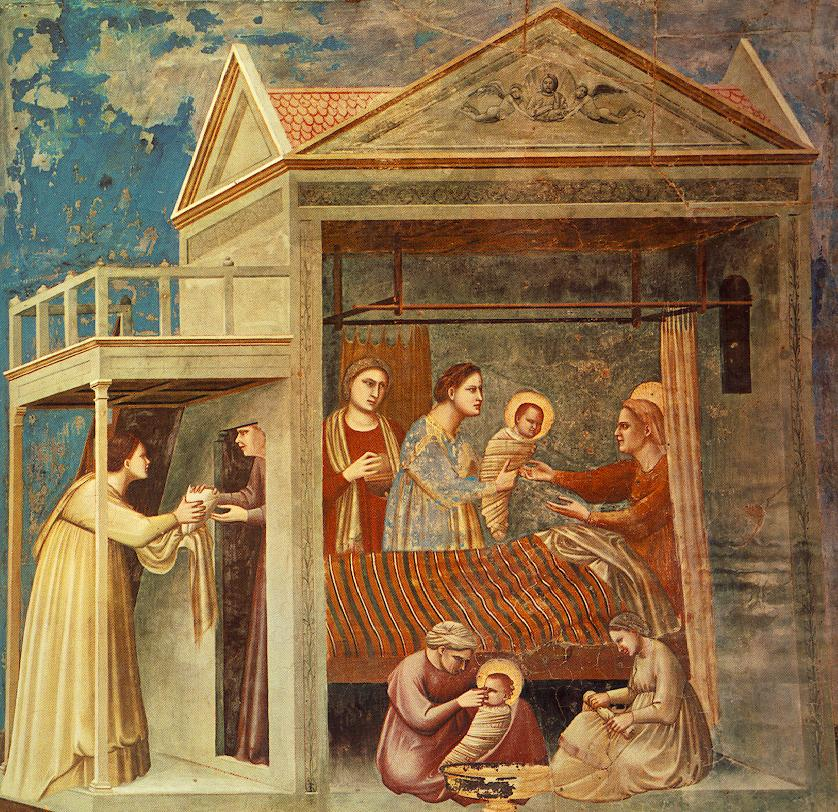
\includegraphics[width=6cm]{imagines/giotto.jpg}
\end{center}

\vfill

Fontes. 
Textus et cantus officii divini secundum 
Antiphonale Monasticum, Solesmis 1933. /
Textus et cantus missæ secundum
Graduale triplex, Solesmis 1979. /
Versus ad communionem secundum
http://media.musicasacra.com/pdf/beatamme.pdf (12.8.2012). /
Translatio capituli sumpta est ex:
Jeruzalémská bible, Praha-Kostelní Vydří 2009. /
Translationes psalmorum ex
Hejčl Jan: Žaltář čili Kniha žalmů, Praha 1922.

Collaborantes.
Textus latinos cantusque transcripsit et omnem laborem typographicum peregit
Jakub Jelínek. /
Proprios cantus festi in linguam bohemicam Jakub Pavlík et Tereza Hodinová
transtulerunt. Pro erroribus autem prior est accusandus. /
Psalmos in lingua bohemica de libro supra dicto transcripsit
Barbora Maturová. /
Filip Srovnal librum istum præparare mandavit et laborem exprobrationibus
utilissimis comitabatur. Ipse etiam neumas super cantus missæ
de Graduali triplici transcripsit. /
Imaginem, quæ paginam tituli ornat, Klára Jirsová pinxit.

Instrumenta adhibita.
LuaTeX, %http://www.luatex.org / 
Gregorio, %http://home.gna.org/gregorio /
typi Junicode. %http://junicode.sourceforge.net

\begin{center}
Liber hic imprimis ad usum chori 
\guillemotright Conventus Choralis\guillemotleft\ 
paratus est
et secundum eius consuetudines.
http://www.introitus.cz

\vspace{1cm}

{\large Editio Sancti Wolfgangi \annusEditionis.}

\vspace{2mm}

Series \guillemotright Conventus\guillemotleft, vol. I.

\vspace{1cm}

http://stiwolfgangi.xf.cz

\end{center}

\vfill

\end{document}
